% !TEX root = main.tex

\section{Ranking the output of Static Analysis}\label{sec:ranking}
% Describing How You Solved the Problem or Answered the Question

% This part of the thesis is much more free-form. It may have one or several sections and subsections. But it all has only one purpose: to convince the examiners that you answered the question or solved the problem that you set for yourself in Section 4. So show what you did that is relevant to answering the question or solving the problem: if there were blind alleys and dead ends, do not include these, unless specifically relevant to the demonstration that you answered the thesis question. 

Given the company context, a single tool approach was chosen as to not introduce extra dependencies/complexity (in contrast to combining different SA tools). 

The different techniques that were tested are:
\begin{itemize}
    \item Using a Bayes Network for prioritizing alerts depending on location information.
    \item Predicting actionable alerts using ML algorithms based on different code/change metrics.
    \item Prioritizing alerts that point at bugs: analyze the code history to see which alerts pointed to fixed bugs and try to extract patterns from that.
    \item Detecting bug-prone methods and prioritizing alerts to those parts of code.
    \item Combining the three aforementioned methods, where each one focuses on a particular part of the dataset/alert types.
\end{itemize}

% Why were these choices made (single tool)?
% Different techniques for different types of alerts (code guidelines vs classical analyzer).
% In this section we present the results of different approaches for ranking static analysis alerts, applied in an industrial codebase.

\subsection{Collecting data}

% Clang tidy - why?\\
Clang AST (\cite{clang_ast}) and Clang Tidy (\cite{clang_tidy}) was used to analyze the code. It was chosen is because it's a reliable open source tool, extensible and most importantly supported by the codebase of the company.

\subsubsection{Clang AST}
Since some of the algorithms need metric data from the code, the Clang AST was chosen to extract that information. Assuming that the project can be successfully compiled, Clang can provide an API on top of the parsed AST.  

All information about the AST for a translation unit is bundled up in the class \textit{ASTContext}, which allows traversal of the whole translation unit.

Clang’s AST nodes are modeled on a class hierarchy that does not have a common ancestor and that consists of three main node types: Declarations, Statements (including Expressions) and Types (each with its own large inheritance hierarchy).

In order to traverse the AST, Clang offers two approaches:
\begin{itemize}
	\item \textbf{RecursiveASTVisitor}: A recursive visitor based approach, which allows you to run custom actions based on the node that is visited.
	\item \textbf{AST Matchers}: An approach that allows you to define what nodes you want to match by using a domain specific language.
\end{itemize}

\subsubsection{Clang Tidy}

Clang Tidy is a modular C++ linter tool which provides an extensible framework for diagnosing and fixing typical programming errors, like style violations, interface misuse, or bugs that can be deduced via static analysis (\cite{clang_tidy}). 

In addition to its Static Analyzer checks, Clang Tidy contains a large list of other checks ranging from those that target bugprone code constructs, to CERT Secure Coding Guidelines, C++ Core Guidelines etc...

Clang Tidy can be configured by selecting the type of checks to be executed or by restricting the parts of code where to carry out such checks.

The following checks were regarded as relevant and used during code analysis:
\begin{itemize}
	\item Clang Static Analyzer checks
	\item Checks related to C++ Core Guidelines
	\item Checks that target bugprone code constructs
	\item Checks related to CERT Secure Coding Guidelines
	\item Checks related to Boost library
\end{itemize}

\subsubsection{Workflow for collecting information \label{data_collection}}

By exploiting the extensibility of Clang Tidy (ability to define new checks) and the power of the Clang AST (collecting information from code), the metrics needed by the ML algorithms can themselves be implemented as checks and thus be extracted automatically when analyzing the codebase. This is a flexible approach which allows to build automatic processing of alerts by integrating alert as well as metric collection within a single toolchain.

In order to make processing alerts easier, the C++ interface code of Clang Tidy was slightly changed to output information in a more suited format (line number instead of bit offset from start of file), hide not useful information, and output alerts only from the file under analysis (not from imported headers).

Starting by the provided open source \href{https://github.com/llvm-mirror/clang-tools-extra/blob/master/clang-tidy/tool/run-clang-tidy.py}{python scripts}, a workflow can be built in python to automatically collect alerts and metrics. In order to crawl the code history of the project, different script were implemented in python to automatically guide the workflow and process the output of SVN (version control system used at the company).

The high level workflow for collecting data consists of the following steps:
\begin{itemize}
    \item Start by selecting a base revision in the code history.
    \item Fully analyze that revision of the codebase (collect all alerts output by Clang Tidy).
    \item Repeat for desired number of iterations (revisions):
        \begin{itemize}
            \item Checkout next revision, detect changed parts of code, collect surrounding information (author, changed methods, etc...).
            \item Run Clang Tidy only on the changed parts of code.
            \item Collect any new alerts and metrics.
        \end{itemize} 
\end{itemize}


\begin{figure}[H]
	\centering
	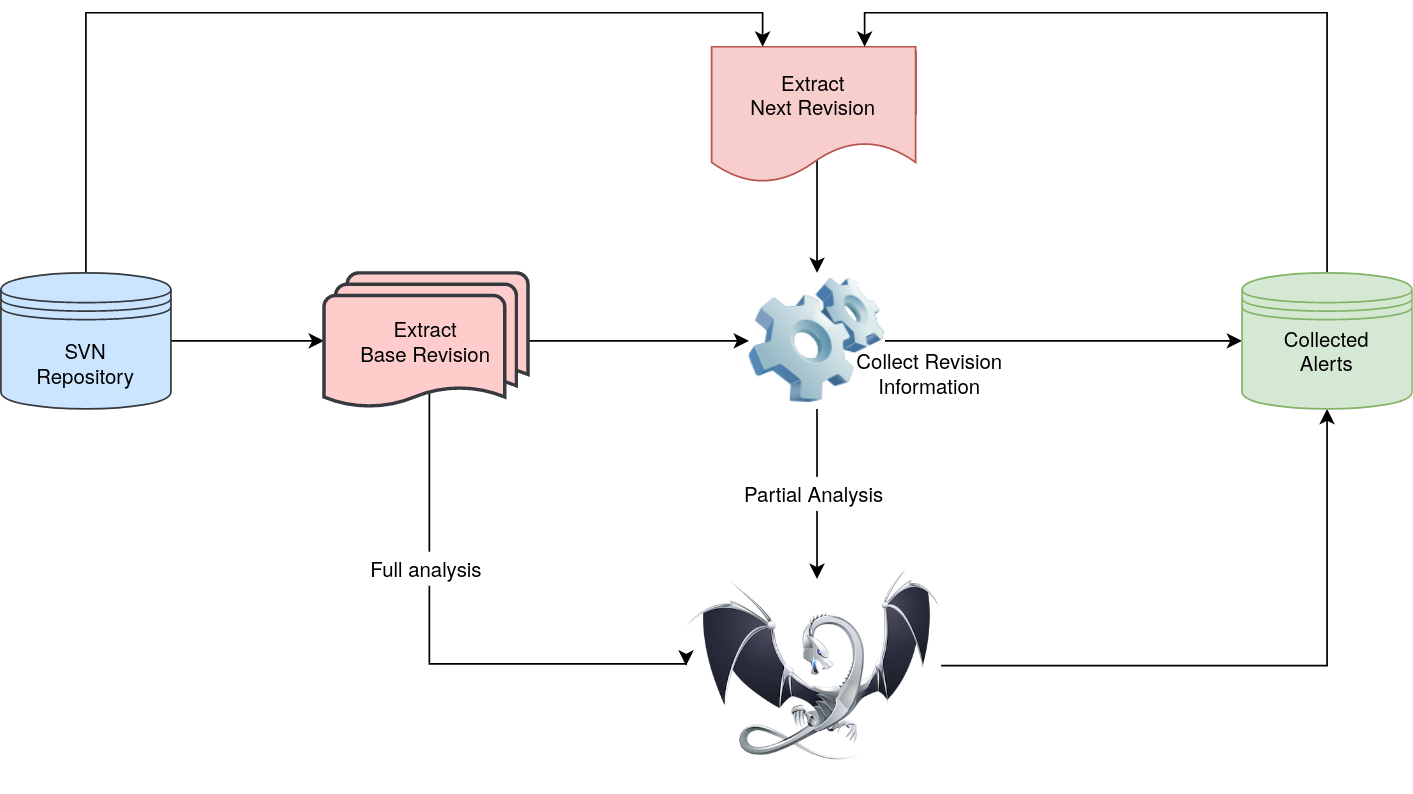
\includegraphics[scale=0.2]{./src/collect_info.png}
	\caption{Collecting alerts and other information}
\end{figure}

\subsubsection{Assumptions made for collected data}
Some algorithms use the notion of Actionable Alerts for processing the output of SA tools. Actionable Alerts (AA) are alerts that are deemed important by developers in the past (alerts that they acted on). In order to automatically label alerts as such (no existing information that can point to that), an important and risky assumption has to be made: alerts that disappear during code changes (revisions/commits) are considered as actionable, the rest is not. 

This assumptions, though necessary, is risky because not all alerts disappear as a result of direct and targeted change by developers. Their disappearance can be caused by other unknown factors (those related to deleted files are not taken into account). Data generated using this approach can contain a lot of false positives and potentially damage the performance of the used ML algorithms.

Another algorithm uses alerts pointing at past bugs as a way to prioritize future alerts. Also in this case an assumption is needed: the alerts that pointed to past bugs, were directly related to that bug. This may not always be true and can cause the aforementioned problems as a result.

The nature of automatic data extraction, without a reliable oracle pointing at the right decisions, leads to impure data and penalizes the efficiency of ML algorithms, but unfortunately it is an indispensable trade-off to be made.

\subsection{Data overview}

\textbf{TODO: Analyze of large portion of revisions and produce statistics}
\textbf{TODO: List which alert types were considered}
\textbf{TODO: Bug statistics for bug related lines}

There are X packages, Y files, Z lines of code.\\
Analyzed X revisions, from Y date to Z date.\\
There are these alerts per type.\\
Open/closed alerts statistics.\\
Alert distribution per type/package (graphs).\\


\subsection{Dealing with unbalanced and noisy data}

Our automatically collected data suffers from two main problems, heavy imbalance and noise. 

Kim et al. \cite{noise_defect} propose a method for dealing with noisy data in the context of defect prediction algorithms. They also provide guidelines for acceptable noise levels and study the impact of different amounts of noise on the prediction performance.
They found out that performance, in terms of f-measure, is affected more by the presence of false positives and that the tested algorithms were robust to the presence of false negatives. When noise levels reach 20-35\% of both FP and FN, the performance decreases significantly, especially on small datasets.
The proposed algorithm for cleaning noisy data by \cite{noise_defect}, calculates the ratio of the top \textit{N} most similar instances of each item that have a different class label. If that ratio exceeds a certain threshold, then that item is considered as noisy.

Batista et al. \cite{balancing_comparison}, perform a comparative evaluation of different dataset balancing techniques. They claim that imbalance alone is not the only reason for poor classifier results, but that it is also related to noisy/overlapping data. According to their experiments, over-sampling methods perform generally better and \textit{SMOTE} + Tomek/ENN provide good results for datasets with few positive examples.

Given the nature of our approach to detecting actionable alerts, it seems plausible that the amount of false positives will be non negligible, and thus there is a high risk that there will be a significant performance impact. Since, the number of examples of the positive class is also rather limited, there seems to be a necessity to apply a combination of balancing and cleaning to the dataset.

\textbf{TO DO: maybe insert before and after graph for data cleaning/balancing?}

\subsection{Feedback Rank and Z-Score}

% \textbf{TODO: maybe try a different correlation (author/alert type/?)}
% check vs naive bayes - trade off with speed

Feedback Rank (\cite{correlation_exploitation}) combined with Z-Score (\cite{z-ranking}) is a simple technique which ranks alerts on the probability of them being true/actionable. It consists of three basic features: package, file, function of the alert being analyzed (though may be extended as needed).
By constructing a Bayesian Network based on these three features and the history of the project (which alerts have been proven valuable) it produces a probability ranking about which alerts are most useful.

As explained on the literature review (\cref{literature}), Feedback Rank is based on the assumption that bugs and false positives are clustered by code locality. The alerts are divided into two major regions, one that contains mostly true positive, and one that contains mostly false positives. A Bayesian Network (BN) is used to calculate the probabilities of an alert or cluster of alerts belonging to a certain region.

\textbf{TODO: add graph of alert distribution for the project, similar to this paper}

The initial configuration of the network can learned from historical data (extracted as explained on \cref{data_collection}). Feedback Rank is supposed to be an online ranking system, if we inspect a report and know its value, the probabilities of the parents are re-calculated.

To construct the BN, the Pomegranate library was used (\cite{pomegranate}), trained with the extracted alert data from the version history.

\textbf{TO DO: used as static, explain zranking assumption, add prediction/train time}


\subsubsection{Z-Score}
To break ties when the probabilities provided by the BN are equal between alerts, the Z-Score metric is used based on the number of alerts on the same file. Z-Score is used in Z-Ranking (\cite{z-ranking}), which makes use of the observation that the most reliable error reports are those that generated few failed checks and many successful checks, since the actual amount of bugs in code is relatively small. 

The \textit{z-test} statistic, which measures how far an observed value is from the real population, in this case produces a large positive \textit{z-score} when there are few errors and many successes, and a large negative \textit{z-score} when there are few successes and many errors.

To make use of the Z-Score, an approximation is made. The granularity used for calculating the scores of alerts is based on file level (how many actionable/unactionable alerts of a certain type in a file), instead of the original granularity of the alert (for example an alert that only works on \textit{for loops}). This approximation is made because we do not know for each alert in which code construct it works on. Also, since it is only used as a tie-breaker, a high precision is not indispensable.

\subsection{Detecting Actionable Alerts via Machine Learning}
% classifiers used, how to train (grid search), overfitting, ways to measure

Different research papers have focused on automatically classifying alerts in true/false positives or actionable/unactionable, by constructing classifiers based on code or change metrics (\cite{actionable_sa}, \cite{model_building_actionable}).

Instead of focusing on classifying alerts as true or false positives, we focus on Actionable Alerts instead: alerts that are deemed important by the developers (not restricted to the type of alerts, but also to the context on which it manifests itself). The later is a less restrictive definition and makes it easier to collect data. Classifying alerts as true or false would necessitate an oracle telling which is which or a large and representative dataset generated manually. In addition, from a developer's perspective, AAs can be more useful. An alert can be true but might be considered not important by developers and thus be equally useless as a false one (low criticality, no impact on user side etc...).

Research is conducted by following the example of \cite{model_building_actionable}, since it contains an agglomeration of alert characteristics (AC) collected from other research papers.

The workflow, as explained in \cref{data_collection}, consists of iterating through the version history, collecting alerts characteristics and keeping track which alerts disappear (considered as actionable). ACs are then later used as features in ML algorithms with actionability being the target to predict.

The scikit-learn library was used to perform ML experiments (\cite{scikit-learn}).

\subsubsection{Alert Characteristics}

The collected ACs can be classified in five main categories: alert information, source code metrics, version history, churn metrics, and aggregate characteristics.

\paragraph{Alert information:} (a) package name (or folder), (b) file name, (c) file extension, (d) alert type, (e) alert category (security, core guidelines...), (f) method signature.

\paragraph{Source code metrics:} (a) number of statements, (b) number of methods, (c) number of classes, (d) cyclomatic complexity.

\paragraph{Version history:} (a) alert open revision, (b) developers who made changes from the open revision of an alert to revision under analysis, (c) file creation revision, (d) file deletion revision, (e) latest modification revision.

\paragraph{Churn metrics:} (a) added lines, (b) deleted lines, (c) growth (added-deleted), (d) total modified (added+deleted), (e) percent modified.

\paragraph{Aggregate characteristics:} (a) total alerts for revision, (b) total open alerts for revision, (c) alert lifetime, (d) file age, (e) alerts for artifact (method, file, package), (f) staleness (amount of time since last change of file, method, package).


\subsubsection{Pre-processing data}

***mostly categorical data -> tree based algorithms\\
\textbf{***do not use label encoding with nominal data (false order)}\\
\textbf{***try other encoding techniques}

\paragraph{Label encoding} Some algorithms need data in numerical form. Since most of the features are categorical data, we need a way to convert them to numerical. A simple approach was chosen, label encoding, which assigns an integer to each value of a category. Other approaches such as One-Hot encoding would increase the amount of data a lot (ex. consider one-hot encoding the file where an alert a method is from, which is a feature with high cardinality).

\paragraph{Imbalanced dataset} A quick look at the number of closed or not closed alerts shows that the dataset is heavily unbalanced. In order to train the ML algorithms we need first to balance the dataset. Two main techniques were tried: random undersampling and SMOTE (by using the library from \cite{imblearn}).\\

\textbf{TO DO:}\\
-cite paper where oversampling works better\\
-list other metrics\\
-explain balancing techniques?

\paragraph{Scaling} While for tree based algorithms scaling is not needed, for other algorithms like Logistic Regression, scaling the inputs can make a difference.

\paragraph{Missing values} In some ACs data may be missing, for example...

\paragraph{Feature selection} The features needed to train the models vary from project to project. Since collecting features that have little to no impact on algorithm performance is a waste of resources, techniques can be applied to select the most representative subset of features. Two main techniques were used: PCA and Recursive Feature Elimination.
\textbf{TODO: COMPARISON FULL FEATURES VS REDUCED}
% correlations?

\subsection{Bug related lines}

Another automatic way to determine which alerts are useful is to check if they pointed to lines that were changed during bug fixes. By doing so, we are regarding as valuable only those alerts that potentially signaled future bugs. The concept of bug related lines (BRL) is used in \cite{which_warnings} and \cite{automatic_training_set}.

BRLs are calculated as follows:
\begin{itemize}
    \item We start at a base revision and iterate backwards to a target revision. 
    \item If revision under analysis is a bug-fixing revision (contains a bug ID) collect changed/deleted code lines from the version history.
    \item If those collected lines were present in the code at least since the target revision, we consider them bug related lines.
    \item Continue iterating backwards, collecting BRLs. If previous lines that were considered BRL were changed before reaching the target revision, we remove them from the set. 
\end{itemize}

\begin{figure}[H]
    \centering
    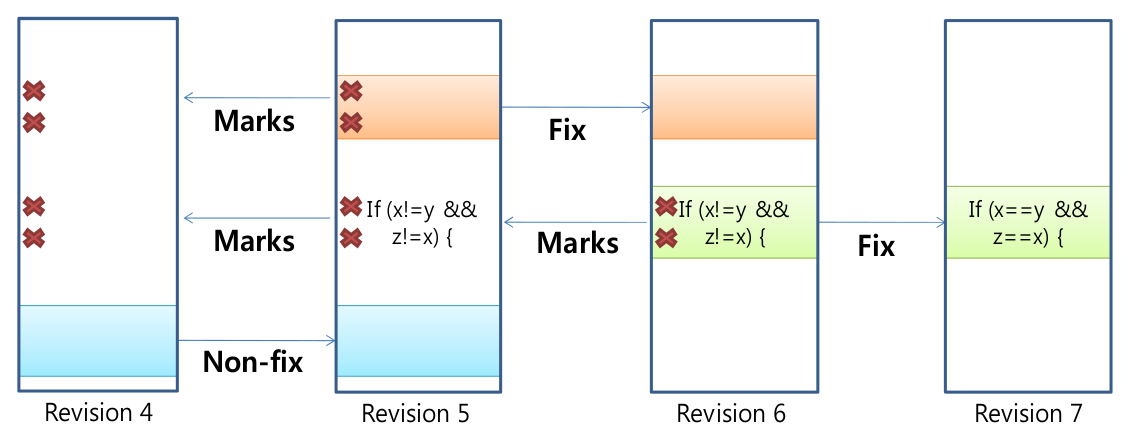
\includegraphics[scale=0.3]{./src/brl_example.png}
    \caption{Calculating BRLs (\cite{which_warnings})}
\end{figure}

% generic BRL vs project specific BRL

Since the amount of collected lines and warnings can be rather limited, we extend the definition to Bug Related Methods (BRM). Namely, we trace in which methods the BRL belong to and also consider alerts inside those methods as valuable. That allows to extend the dataset, but also potentially weakens the data by introducing more noise.

Given that the number of alerts collected this way, is a lot less than the total number of alerts, this method is more suited for ranking alert types rather than individual alerts (as used in \cite{which_warnings}).

\begin{figure}[ht]
	\centering
	\begin{minipage}{.5\linewidth}
		\begin{algorithm}[H]
			\SetAlgoLined
			\KwData{Collected bug-related alerts}
			\KwResult{Weighted alert types}
			$\alpha, \beta = x, y$\;
			$w_t = 0 \ for \ t \ in \ alertTypes$\;
			\For{alert in collectedAlerts}{
				$w_t = typeOf(alert)$\;
				\If{alert pointed to a BRL}{
					$w_t = w_t + \alpha$
				}
			
				\ElseIf{alert pointed to a BRM}{
					$w_t = w_t + \beta$
				}
			}
			\caption{Alert type priotitization algorithm}
		\end{algorithm}
	\end{minipage}
\end{figure}

\subsection{Bug prediction}

Following the example of \cite{static_profiling}, which aims to prioritize alerts based on the execution likelihood of the code pointed by the alert, we present a similar approach. Alerts pointing at potential bugs are the ones that can be considered the most important. The cost of detecting and fixing a bug is much lower if detected early in the development cycle. If we can predict which components will be likely to cause failures in the future, we can prioritize alerts that point to those components. 

The appropriate granularity to use for bug prediction is at method level. File level granularity is too broad since a lot of files contain many lines of code, which would result in prioritizing a lot of alerts, while anything lower than method level would be too hard to predict as bug prone.

We follow the example of the \cite{prediction_method} method. By using a combination of source code and change metrics and by exploiting the version history of the codebase, classifiers can be built that predict bug prone methods.

\begin{table}[H]
	\centering
	\begin{tabular}{@{}ll@{}}
		\textbf{Metric Name}          & \textbf{Description}                                                                                                                   \\ \midrule
		\textit{methodHistories}      & Number of times a method was changed                                                                                                   \\ \midrule
		\textit{authors}              & Number of distinct authors that changed a method                                                                                       \\ \midrule
		\textit{stmtAdded}            & Sum of all source code statements added to a method                                                                                    \\ \midrule
		\textit{maxStmtAdded}         & \begin{tabular}[c]{@{}l@{}}Maximum number of source code statements added \\ \\ to a method body for all method histories\end{tabular} \\ \midrule
		\textit{avgStmtAdded}         & \begin{tabular}[c]{@{}l@{}}Average number of source code statements added\\ to a method body per method history\end{tabular}           \\ \midrule
		\textit{stmtDeleted}          & \begin{tabular}[c]{@{}l@{}}Sum of all source code statements deleted from\\ a method body over all method histories\end{tabular}       \\ \midrule
		\textit{maxStmtDeleted}       & \begin{tabular}[c]{@{}l@{}}Maximum number of source code statements\\ deleted from a method body for all method histories\end{tabular} \\ \midrule
		\textit{avgStmtDeleted}       & \begin{tabular}[c]{@{}l@{}}Average number of source code statements\\ deleted from a method body per method history\end{tabular}       \\ \midrule
		\textit{churn}                & \begin{tabular}[c]{@{}l@{}}Sum of stmtAdded - stmtDeleted over all\\ method histories\end{tabular}                                     \\ \midrule
		\textit{maxChurn}             & Maximum churn for all method histories                                                                                                 \\ \midrule
		\textit{avgChurn}             & Average churn per method history                                                                                                       \\ \midrule
		\textit{decl}                 & \begin{tabular}[c]{@{}l@{}}Number of method declaration changes over all\\ method histories\end{tabular}                               \\ \midrule
		\textit{cond}                 & \begin{tabular}[c]{@{}l@{}}Number of condition expression changes in a\\ method body over all revisions\end{tabular}                   \\ \midrule
		\textit{elseAdded}            & \begin{tabular}[c]{@{}l@{}}Number of added else-parts in a method body\\ over all revisions\end{tabular}                               \\ \midrule
		\textit{elseDeleted}          & \begin{tabular}[c]{@{}l@{}}Number of deleted else-parts from a method\\ body over all revisions\end{tabular}                           \\ \midrule
		\textit{cyclomaticComplexity} & Current cyclomatic complexity of method                                                                                                \\ \midrule
		\textit{nestingDepth}         & Current nesting depth of method                                                                                                        \\ \midrule
		\textit{totalStatements}      & Current number of statements in method                                                                                                 \\ \midrule
		\textit{nrPaths}              & Current number of paths in method                                                                                                      \\ \midrule
		\textit{nrDeclarations}       & Current number of declarations in method                            \\\midrule 
	\end{tabular}
\end{table}

% rank alerts in problematic zones higher - combine with BRL?

\subsection{Combining the techniques}
% \subsection{Individual alert tuning}
% zranking cppcore guidelines
% COMBINE DIFFERENT TECHNIQUES FOR DIFFERENT ALERTS

\subsubsection{How to combine the strengths?}
% deep learning? make it flexible, learn with time\\
apply each technique to a subset of the warnings (which is more appropriate)

\subsubsection{Better results?}
Does it provide better results?


\subsection{Evaluation methods}

To evaluate and compare the approaches different techniques are used: 
\begin{itemize}
    \item \textbf{K-Fold Cross Validation}: where the data is randomly divided into folds and one of those is used for testing while the rest for training. It is often used in papers containing ML approaches to ranking alerts, though it has its drawbacks. As shown in \cite{performance_method_bug} and as can be seen on \cref{kfold_vs_release}, this approach uses dependent variables (most of the extracted features), that may not be available at prediction time in a real world scenario. That can lead to unreliable and excessively optimistic results.
    \item \textbf{Release/Revision based testing}: avoids the drawback of the previous method, by using a \textit{"horizontal"} train/test strategy. We fix a certain point in time (revision or release) which defines what the train set (before that point) and test set (after that point) will be. This trains the algorithms with more realistic data, but it also has its drawbacks. In a scenario where the dataset is imbalanced, a \textit{"horizontal"} 80/20\% split may leave us with very little data. Also, unlike in cross validation, we cannot train and test different models.
    \item \textbf{Alert ratio}: where we compare how much better is the ranking produced by a model with a random order of alerts. We calculate that by checking how many more alerts are better placed in the ranked version than the random one.
    \item \textbf{Average inspected false positives}: similar to the previous method where we compare the ranking produced by a model against a random one, but by calculating the average  number of times an unactionable alert has to be inspected before reaching an actionable one.
    \item \textbf{Fault detection rate curve}: the curve of a model is formed by the percentage of all actionable alerts found within the first \textit{X} alerts of the alert
    ranking algorithm.
    
    TO DO: see \cite{compare_framework} and apply only on top x\%? Fault detection rate curve?
    
    % \item Feedback-Rank paper has some approaches.
\end{itemize}

\begin{figure}[H]
    \centering
    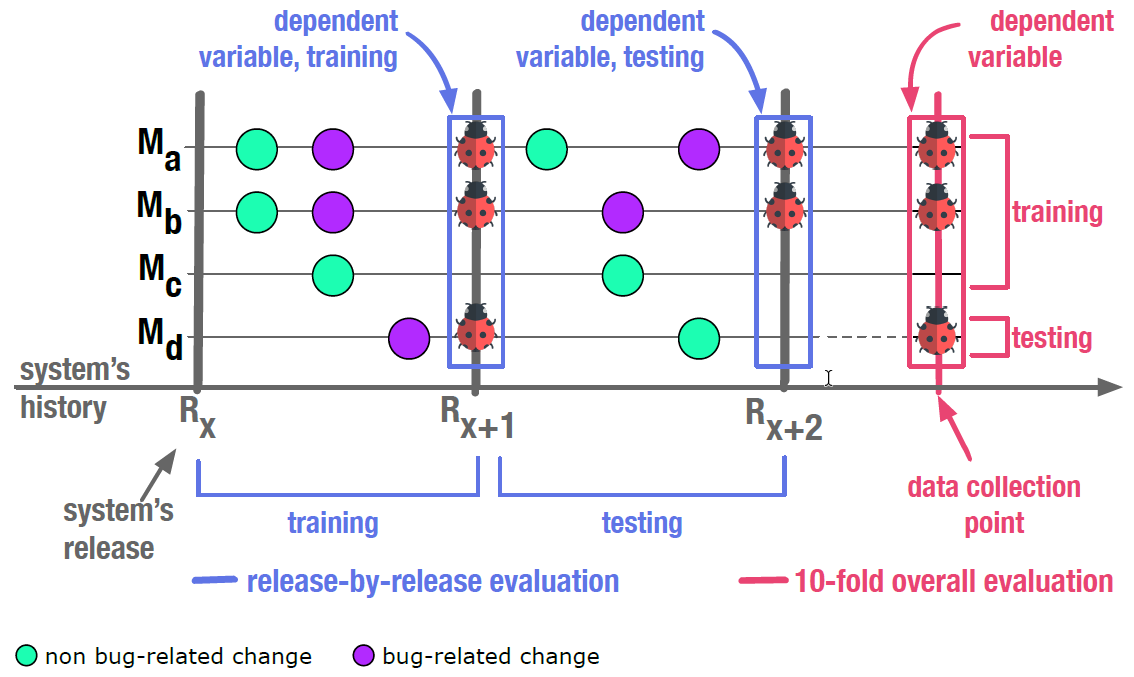
\includegraphics[scale=0.3]{./src/release_based_testing.png}
    \caption{Release-based vs K-Fold (\cite{performance_method_bug})}
    \label{kfold_vs_release}
\end{figure}

\subsubsection{Evaluation Metrics}

Along with the classic evaluation metrics like \textit{accuracy}, \textit{precision} and \textit{recall}, other metrics are used that are more appropriate for imbalanced data (\cite{comparison_metrics}, \cite{iba_metric}). 


\begin{gather*}
Sensitivity = \frac{TP}{TP + FN}\\
Specificity = \frac{TN}{FP + TN}\\
G-Mean = \sqrt{Sensitivity * Specificity}
\end{gather*} 
Sensitivity, or True Positive Rate is the percentage of positive examples which
are correctly classified.\\
Specificity, or True Negative Rate, is the percentage of negative examples which are correctly classified.\\
G-Mean is the geometric mean of the sensitivity and specificity.


\begin{gather*}
AUC = \frac{Sensitivity + Specificity}{2} \qquad (*approximation \ using \ trapezoid \ rule)
\end{gather*} 
The \textit{AUC} of a binary classifier is equivalent to the probability that the classifier will rank a randomly chosen positive instance higher than a randomly chosen negative instance.


\begin{gather*}
IBA_{\alpha} = (1 + \alpha * (Sensitivity - Specificity)) * Sensitivity * Specificity
\end{gather*} 
The \textit{Index of Balanced Accuracy} used for evaluating learning processes in two-class imbalanced domains. The
method combines an unbiased index of its overall accuracy and a measure about
how dominant is the class with the highest individual accuracy rate.


\subsubsection{Preparing the dataset}
Since the amount of actionable warnings is very low compared to the total amount of warnings, the dataset is balanced in two steps. First a subset of the packages and warnings is selected. By considering the ratio of actionable to the total amount of alerts, we can select the packages or types of warnings with the higher ratio (ex. the first 100).

After the first step, a test set is selected for evaluating the algorithms (equal to 20\% of the dataset).
That is especially needed to test the algorithms after the K-Fold evaluation.

The second step consists of balancing the amount of actionable and not actionable alerts, either by random subsampling or by artificially creating new samples (via SMOTE).


\textbf{TODO: EVALUATE OVERSAMPLING METHODS}

\textbf{TODO: EVALUATE ENCODING METHODS}

\subsection{Results of individual tools}

\subsubsection{Random test set}
\subsubsection{Release based testing}
\subsubsection{Alert ratio}
\subsubsection{Average false positives to inspect}


% results of each tool\\
% how to prepare a fair dataset:  normal vs release based\\
% personal feedback


% \section{Other approaches}

% \subsection{Other stuff}
% execution analysis?\\
% ir for bug messages


